\newcommand{\doctitle}{Construct and Destroy \\ Software Architecture}
\newcommand{\doctitleshort}{C\&D Software Architecture}

\newcommand{\docauthor} {
    \renewcommand{\arraystretch}{0.5}
    \begin{tabular}{l l}
        \textbf{Students:} & ~ \\
        Mark van der Woude     & {\mdseries(S1081655)} \\
        Stephan Schrijver     & {\mdseries(S1078783)} \\
        Jeroen Vinke     & {\mdseries(S1078666)} \\
        Sander Bouwman   & {\mdseries(S1080528)} \\
        Robin T. Koning  & {\mdseries(S1078710)} \\
    \end{tabular}
}

\newcommand{\doctitlepage} {
    \thispagestyle{empty}
    \parbox[t]{1.0\linewidth}{
        \fontsize{40pt}{60pt}\selectfont
        \vspace*{1.5cm}
        \doctitle{}
        \vspace*{1.5cm}
    }
    \vfill
    {
        \centering
        \large
        \hfill \today
        \hfill \docauthor{}
    }
    \normalcolor{}

    \newpage
}

\providecommand{\doctitle}{Title}
\providecommand{\docauthor}{Author}
\providecommand{\doctype}{scrartcl}
\providecommand{\doctitlepage}{TitlePage}

\documentclass[12pt,a4paper,titlepage,parskip=full]{\doctype}

\usepackage[english]{babel}
\usepackage{caption}
\usepackage{float}
\usepackage{blindtext}
\usepackage{hyperref}
\usepackage{graphicx}
\usepackage{listings}
\usepackage{tikz}
\usetikzlibrary{decorations.pathreplacing}
\usepackage{pdfpages}
\usepackage{apacite}
\bibliographystyle{apacite}

% set Listing settings -------------------------------------
\usepackage{listings}
\usepackage{color}

\lstset{frame=tb,
  language=C++,
  backgroundcolor=\color{black!5}, % set backgroundcolor
  aboveskip=3mm,
  belowskip=3mm,
  showstringspaces=false,
  columns=flexible,
  basicstyle={\small\ttfamily},
  numbers=none,
  numberstyle=\tiny\color{gray},
  keywordstyle=\color{blue},
  commentstyle=\color{dkgreen},
  stringstyle=\color{mauve},
  breaklines=true,
  breakatwhitespace=true,
  tabsize=3
}



% Input and output encoding ---------------------------------------------------
\usepackage{iftex}
\ifPDFTeX
   \usepackage[utf8]{inputenc}
   \usepackage[T1]{fontenc}
   \usepackage{lmodern}
\else
   \ifXeTeX
     \usepackage{xltxtra}
   \else
     \usepackage{luatextra}
   \fi
   \defaultfontfeatures{Ligatures=TeX}
\fi

% Math
\usepackage{amsmath}
\usepackage{amsfonts}
\usepackage{amsthm}
\usepackage{amssymb}
\usepackage{mathtools}
\usepackage{bm}
\newcommand{\uvec}[1]{\boldsymbol{\hat{\textbf{#1}}}}

\DeclarePairedDelimiter{\ceil}{\lceil}{\rceil}
\DeclarePairedDelimiter{\floor}{\lfloor}{\rfloor}
\DeclarePairedDelimiter{\bag}{\langle}{\rangle}
\DeclarePairedDelimiter{\set}{\{}{\}}

% Misc
\usepackage{marginnote}
\usepackage[shortlabels]{enumitem}

% Display
\usepackage{lastpage}
\usepackage{fancyhdr}
\setlength{\headheight}{24pt}
\usepackage{eurosym}
\pagestyle{fancy}

\usepackage[nameinlink]{cleveref}

\title{\doctitle}
\author{\docauthor}
\date{\today}

\lhead{\doctitleshort}
\rhead{\today}
\cfoot{\thepage\ /~\pageref{LastPage}}
%\lfoot{\docauthor}

\numberwithin{equation}{section}
\numberwithin{figure}{section}
\numberwithin{table}{section}

\usepackage{changepage}

%Other settings
\lstset{basicstyle=\ttfamily}

\begin{document}
\doctitlepage{}

\tableofcontents
\thispagestyle{empty}
\newpage

\clearpage
\setcounter{page}{1}
\addtocontents{toc}{\protect\thispagestyle{empty}}
\newpage

% Abstract, the intro to our document
\begin{abstract}
\blindtext
\end{abstract}

\newpage

%----------------------------------
% Put new chapters in this block

\section{Selection} In this chapter we will explain how our selection system
works. We will show which classes are involved and how the methods are chained
using UML-diagrams. 

\subsection{User interface} First off, how does the selecting feature works.
You can select a unit by clicking on it using the left mouse button. You can
select multiple by holding the left mouse button and dragging, while dragging a
rectangle is drawn. This rectangle represents the selecting area. When you
release the left mouse button every unit in the selecting area, the red
rectangle, will be selected. A selected unit is recognizable by the red line
around it.

\subsection{Selection process} First we made a handler that handles mouse input
for a panel that represents the world in the user interface. This is the
MouseHandler class, it derives from the SDL\_MouseEventSlot class which derives
from the Slot class. The SDL library provides us with low level access to the
mouse input on the window.  The header file of the MouseHandler can be found 
at \cref{lst:mousehandlerheader}.

\begin{lstlisting}[caption={Mouse handler header file.},
label={lst:mousehandlerheader}]
class MouseHandlerWorld : public SDL_MouseEventSlot {
private: 
    int start_drag_x; 
    int start_drag_y;
    void handle_up(sdl_mouse_event_data data); 
    void handle_down(sdl_mouse_event_data data); 
    void handle(sdl_mouse_event_data);
    void handle_motion(sdl_mouse_event_data);
    void handle_left_button(const vec2 &); 
    void handle_right_button(sdl_mouse_event_data &, const vec2 &);

public: 
    MouseHandlerWorld(); 
    ~MouseHandlerWorld(); 
    void on(sdl_mouse_event_data d) override; 
}; 
\end{lstlisting}

The class has a lot of private methods that handle the different types of mouse
events. It has one method that has been overridden from the base class, which
is the on-method. The on-method is where user inputs comes in. In this method
the input is separated into two groups and will be handled further by other
methods. To make it clear how this works an explanatory activity diagram can be
found at \cref{fig:activitymousehandler} in the appendix to illustrate the
process. 

After the on-method has determined whether the incoming data is a motion event
or button it will be handled further by other methods. We will start with the
motion input.

Motion input is handled by the handle\_motion method. Motion is only
important for us when the user is dragging. This means the user is holding the
left mouse button down while moving the mouse. When the user is dragging we set
the position the mouse has moved to and let the UI component know that the user
is dragging by setting a variable dragging to true. The UI component has two
methods called draw\_selection\_rectangle and render. Whenever the render
method is called and the variable dragging is true it will call the
draw\_selection\_rectangle with the positions set by the last call to the 
handle motion method.

Button input is handled a bit differently since we first need to determine what
kind of event it is and from which button. If the event comes from the right
button, it is an event that will control units. Since that has nothing to do
with this topic we will leave it there and explain it in a different chapter. 

If, however, the event does come from the left button it is to select units. 
When the left button is pressed down we get the position of the cursor. 
This will be the starting position of the selection rectangle. After a button 
down event from the left button, a button up event will inevitably be fired 
from the button. This event means a few things. First off all the user has 
stopped dragging, because we stated earlier that the user is dragging when he's 
holding down the left button. So we set the dragging variable to false. Also we 
reset the positions to be ready for a next drag event. After resetting the 
variables, we call the handle\_up method. This determines whether the event 
was a drag or a click of the left mouse button. A click is when you press and 
release the mouse in the same position or at maximum 10 pixels away from the 
original position. We have implemented it this way so it is easier to click 
moving targets. The handle\_left\_button\_click is called and it selects the 
target on the clicking position, unless there is no target in range.

When you release the left mouse button more than 10 pixels away from the origin
point you are dragging the mouse. The position of the release of the button and
the position of the press will passed to the select\_units\_in\_rectangle
method. The method first calculates the right, left, upper and bottom offsets 
for the rectangle. After this all units inside will be selected by checking 
which of the units that belong to the player are positioned inside the 
rectangle. At \cref{fig:selectiondrag} you can find a picture of a few 
units that are selected by the select\_units\_in\_rectangle function and you 
can also see the red rectangle that has been used to select them. 

\begin{figure}[H] 
    \centering
    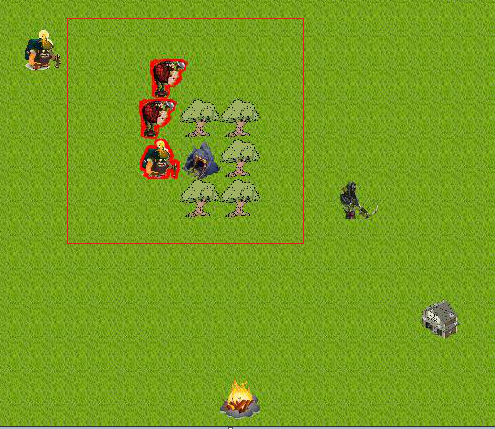
\includegraphics[scale=1.0]{res/SelectionRectangle.png} 
    \caption{Selection by dragging the mouse.}\label{fig:selectiondrag}
\end{figure} 

\newpage

%----------------------------------

\bibliography{bib/sources}
\newpage

\section{Appendix}
\begin{figure}[!htb]
    \centering
    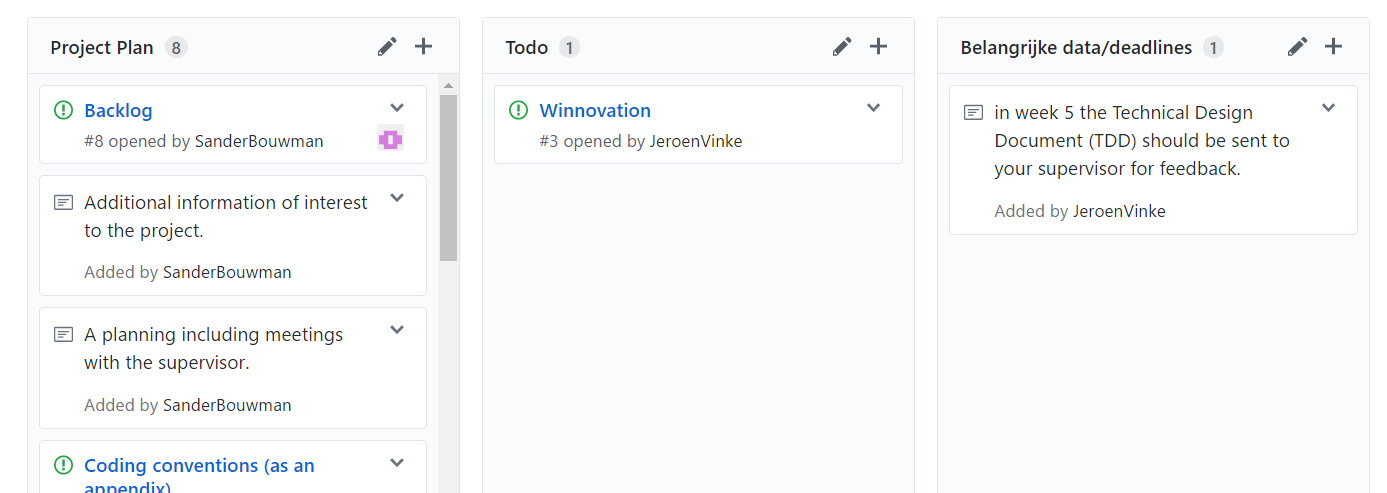
\includegraphics[angle=-90,origin=c,scale=0.75]
    {images/github-projects.PNG}
    \caption{GitHub project}\label{fig:githubproject}
\end{figure}

\end{document}

